\documentclass[]{beamer}
\usepackage[utf8]{inputenc}
\usepackage{xeCJK}
\usepackage{graphicx}
\usepackage{subfigure}
\usepackage{mathtools}
\usepackage{utopia} %font utopia imported
\usetheme{CambridgeUS}
\usecolortheme{dolphin}
\usefonttheme{professionalfonts}
\usepackage{natbib}
\usepackage{hyperref}
\usepackage{fontspec}
\usepackage{setspace}
% \usepackage{enumitem}

\setCJKmainfont{SourceHanSansSC-Regular.otf}[Path=../, BoldFont=bold.otf]

\setbeamerfont{title}{size=\Large}
\setbeamerfont{subtitle}{size=\small}
\setbeamerfont{date}{size=\small}
\setbeamerfont{institute}{size=\small}

\setstretch{1.3}
% \setlength{\parindent}{2em}
% \setlength{\parskip}{0pt}

% \setlist[itemize]{leftmargin=2em}

% ↓↓↓ Modify this ↓↓↓
\title{高等数学I\quad 习题课02}
\subtitle{数学证明}
\date[2025.9.25]{2025.9.25}
% ↑↑↑ Modify this ↑↑↑

\author[上海科技大学]{}
\institute[]{上海科技大学}



\begin{document}

\begin{frame}
    \vspace{15pt}
    \titlepage
\end{frame}

\begin{frame}{Quiz}
    \[
    \text{\Huge 18:00 - 18:20}
    \]
\end{frame}

\begin{frame}{目录}
    \tableofcontents
\end{frame}

\AtBeginSection[ ]
{
\begin{frame}{目录}
    \tableofcontents[currentsection]
\end{frame}
}

% ↓↓↓ Modify From This ↓↓↓
\section{简介}

\begin{frame}{Late Welcome}
    \begin{itemize}
        \item 高数(乃至几乎所有其他课程)的节奏都很快...
        \item 调整好自己的节奏,及时向他人寻求帮助
        \item \textbf{Participate,Ask, Try}.
    \end{itemize}

    \vspace{0.5cm}
    \centering
    \textit{“Better late than never!”}
\end{frame}

\begin{frame}{习题课?}
    \begin{itemize}
        \item 作为高等数学I课程的一部分
        \item Quiz将利用习题课时间进行,会提前通知
        \item 讲以下内容:
        \begin{itemize}
            \item 作业,Quiz
            \item 课堂知识回顾与拓展
            \item etc.
        \end{itemize}
        \item 习题课是对课堂、课本内容的\textbf{补充}而非重复
    \end{itemize}
\end{frame}


% \begin{frame}{投票}
%     \begin{itemize}
%         \item 在课程过程中出现,用以检测大家对知识的理解程度
%     \end{itemize}
%     \vspace{200pt}
    
% \end{frame}

\section{直接证明 / Direct Proofs}

\begin{frame}{简例}
    定理:如果$n$是偶数,那么$n^2$也是偶数.
    
    证明:令$n$为偶数,则其可写为$n=2k$,其中$k$为整数.

    \hspace{3em} 则$n^2=(2k)^2=4k^2=2(2k^2)$.

    \hspace{3em} $2k^2$是整数,故存在一个整数$m=2k^2$,使得$n^2=2m$.

    \hspace{3em} 因此$n^2$是偶数.$\square$
\end{frame}

\begin{frame}{直接证明法}
    \begin{itemize}
        \item 为了证明命题 $P\Rightarrow Q$,我们:
        \begin{itemize}
            \item 假设$P$成立
            \item 运用逻辑推理从$P$推导得到$Q$
            \item 成功了!
        \end{itemize}
        \item 但是一定只能直接证明$P\Rightarrow Q$吗?
    \end{itemize}
\end{frame}

\section{间接证明 / Indirect Proofs}

\begin{frame}{等价命题}
    \begin{itemize}
        \item 考虑$P\Rightarrow Q$的等价命题:\[
        P \Rightarrow Q = \neg P \vee Q = \neg(\neg Q) \vee (\neg P) = \neg Q \Rightarrow \neg P
    \]
    \end{itemize}
    \begin{itemize}
        \item 因此,证明$\neg Q \Rightarrow \neg P$也可证明欲证命题.
    \end{itemize}
\end{frame}

\begin{frame}{简例}
    定理:如果$n^2$是偶数,那么$n$也是偶数.
    
    证明:反证法.尝试证明:若$n$是奇数,那么$n^2$也是奇数.

    \hspace{3em} $n=2k+1,k\in \mathbb{Z}$,
    
    \hspace{3em} 故$n^2=(2k+1)^2= 4k^2+4k+1=2(2k^2+2k)+1$

    \hspace{3em} $2k^2+2k\in\mathbb{Z}$,故$\exists m\in\mathbb{Z}, m=2k^2+2k$,使得$n^2=2m+1$.

    \hspace{3em} 因此$n^2$是奇数.$\square$
    
\end{frame}

\begin{frame}{反证法}
    \begin{enumerate}
        \item 声明该证明使用反证法
        \item 写出逆否命题
        \item 证明逆否命题
    \end{enumerate}
    思考:可否在反证法里嵌套反证法?
\end{frame}

\begin{frame}{典例:$\sqrt{2}$是无理数}

假设$\sqrt{2}$是有理数,则其可以表示为两个互质的正整数$p,q$之比
        \[
        \sqrt{2}=\frac{p}{q} \Rightarrow p^2=2q^2
        \]
则$p^2$是偶数(因为$q^2$是整数),因此$p$也是偶数(反证法).因此可有$p=2k, k\in\mathbb{Z}$. 代回,有$4k^2=2q^2$,则$q$也是偶数.

$p,q$均为偶数,与最初的假设\textbf{矛盾},故$\sqrt{2}$是无理数.$\square$
  
\end{frame}

\begin{frame}{反证法的分类}
    \begin{enumerate}
        \item 证明逆否命题法 \textit{Proof by Contrapositive}
        \begin{itemize}
            \item 证明与原命题完全等价的逆否命题,从而证明原命题
        \end{itemize}
        \item 归谬法 \textit{Proof by Contradiction}
        \begin{itemize}
            \item 假设命题不成立
            \item 通过推理得到矛盾
            \item $\Rightarrow$ 最初的假设错误,则欲证命题成立
        \end{itemize}
    \end{enumerate}
\end{frame}

\section{数学归纳法 / Induction}

\begin{frame}{科学归纳与数学归纳}
    \begin{itemize}
        \item 科学归纳法:
        
        $\rightarrow$ 进行一系列实验,找出能解释所有结果的规律.
        
        \hspace{1em} 即使所有数据都正确,\textbf{结论也可能错误}.

        \item 数学归纳法:
        
        $\rightarrow$ 从一系列被假定为真的陈述开始,运用逻辑推理证明某个结论必然成立.

        \hspace{1em} 若所有初始假设均正确,则结论\textbf{必然正确}.

    \end{itemize}
\end{frame}

\begin{frame}{数学归纳法}
    \begin{itemize}
        \item 一种证明技巧
        \begin{itemize}
            \item 基础步骤:证明命题在某个初始值(常为$n=1$或$n=0$)成立
            \item 归纳假设:$\forall k \in \mathbb{D}$,假设命题在$n=k$时成立
            \item 归纳步骤:证明命题在$n=k+1$时成立
        \end{itemize}
    \end{itemize}
\end{frame}

\begin{frame}{数学归纳法}
    \begin{itemize}
        \item 多米诺骨牌
    \end{itemize}
    \begin{figure}[H]
        \centering
        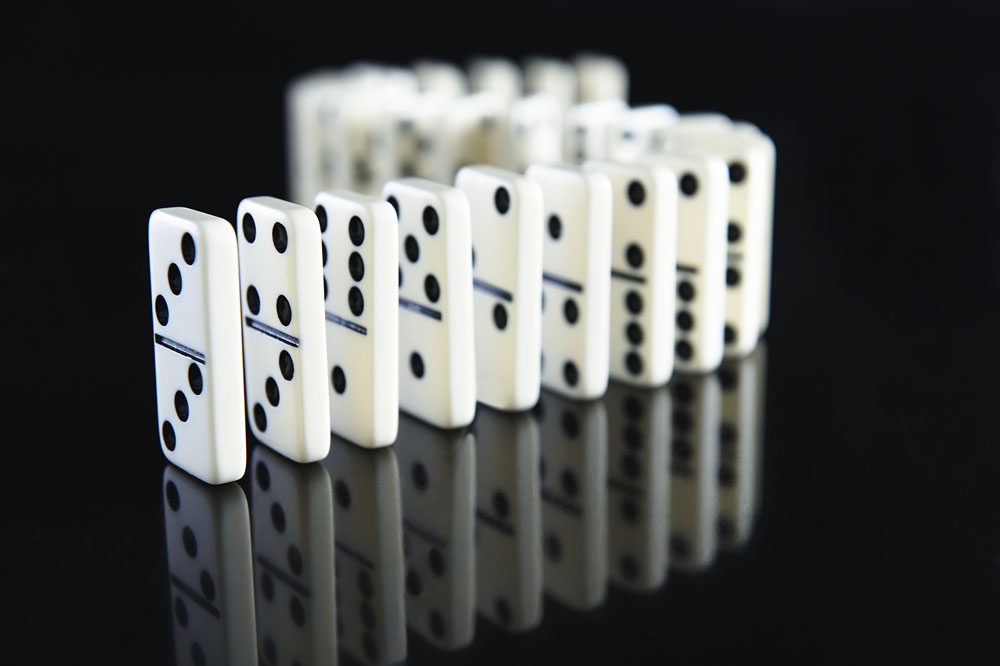
\includegraphics[width=0.7\linewidth]{induction1.jpg}
    \end{figure}
\end{frame}

\begin{frame}{数学归纳法}
    \begin{enumerate}
        \item 确保骨牌之间架设合理(前一张倒下能够使得后一张也倒下)
        \item 推倒第一张骨牌
    \end{enumerate}
    \(\Rightarrow\) 所有骨牌都可倒下\\
    \vspace{5pt}
    在实际证明中,我们常常将这两个步骤顺序进行调换.
\end{frame}

\begin{frame}{流程}
    \begin{itemize}
        \item 对于一个命题\(P(n)\),想要证明其对所有\textbf{(有限的)}自然数$n$均成立\\
        \textit{(思考:为什么一定要是有限的?)}
        \item 分别证明:
        \begin{enumerate}
            \item $P(0)$ 或 $P(1)$ 成立(即初始情况成立)
            \item 假设 $P(k)$ 成立,则\(P(k)\Rightarrow P(k+1)\)
        \end{enumerate}
    \end{itemize}
\end{frame}

\begin{frame}{例}
    \begin{itemize}
        \item 证明:\\
    \ \ \ \ 对于所有的\(n\in\mathbb{N}^*\),
    \end{itemize}
    \[
    \sum_{i=1}^nn^2=1^2+2^2+3^2+\cdots+n^2=\frac{n(n+1)(2n+1)}{6}
    \]
    
\end{frame}

\begin{frame}{思考}
    \hspace{2em}以这样的方式归纳,一定能得到正确的结论吗?
\end{frame}

\begin{frame}{反例1:所有的马的颜色都相同}
    \hspace{2em} 命题:一个人观察到的前$n$匹马都是同一个颜色的
    \begin{itemize}
        \item 基本情况:1匹马 \textit{Trivial}
        \item 归纳假设:假设有$n$匹马都是同一个颜色
        \item 归纳证明:对任意$n+1$匹马:
        \begin{itemize}
            \item 排除第1匹马,剩余的$n$匹马都是同一个颜色
            \item 排除第$n+1$匹马,剩余的$n$匹马都是同一个颜色
        \end{itemize}
        $\Rightarrow$ 所有马都是同一个颜色 
        \item 错在哪里?
    \end{itemize}
\end{frame}


\begin{frame}{反例1:所有的马的颜色都相同}
    \hspace{2em} 命题:一个人观察到的前$n$匹马都是同一个颜色的
    \begin{itemize}
        \item 基本情况:1匹马 \textit{Trivial}
        \item 归纳假设:假设有$n$匹马都是同一个颜色
        \item 归纳证明:对任意$n+1$匹马:
        \begin{itemize}
            \item 排除第1匹马,剩余的$n$匹马都是同一个颜色
            \item 排除第$n+1$匹马,剩余的$n$匹马都是同一个颜色
        \end{itemize}
        $\Rightarrow$ 所有马都是同一个颜色 
        \item 从1匹马至2匹马的推论不成立
    \end{itemize}
\end{frame}

\begin{frame}{反例2:调和级数是收敛的}
    \begin{itemize}
        \item 调和级数:$\sum\limits_{n=1}^{\infty}\frac{1}{n}$ (发散性证明:第零章讲义p8)
        
        \item 错证:
        \begin{itemize}
            \item 初始情况:$n=1, S=1$,极限存在
            \item 假设$n=k$时,调和级数的部分和($1+\frac12+\cdots+\frac1n$)极限存在
            \item 那么这个部分和再加$\frac{1}{n+1}$的极限一定也存在
            \item 因此对于所有的$n$,调和级数的值都确定且不为无穷.收敛!
            
        \end{itemize}
        \item 错在哪里?
    \end{itemize}
\end{frame}


\begin{frame}{反例2}
        \begin{itemize}
        \item 调和级数:$\sum\limits_{n=1}^{\infty}\frac{1}{n}$ (发散性证明:第零章讲义p8)
        
        \item 错证:
        \begin{itemize}
            \item 初始情况:$n=1, S=1$,极限存在
            \item 假设$n=k$时,调和级数的部分和($1+\frac12+\cdots+\frac1n$)极限存在
            \item 那么这个部分和再加$\frac{1}{n+1}$的极限一定也存在
            \item 因此对于所有的$n$,调和级数的值都确定且不为无穷.收敛!
            
        \end{itemize}
    \end{itemize}
    \begin{itemize}
        \item 使用数学归纳法证明一个命题在$n=\infty$处的性质时,需要额外证明该命题在无穷处不失效.
    \end{itemize}
\end{frame}

\begin{frame}{反例3:数列$a_n=2^n$的前$n$项和是$2^{n+1}$}
    \begin{itemize}
        \item 假设当$n=k$时,$\sum\limits_{n=1}^k 2^n=2^{n+1}$ 即命题成立.
        \item 当$n=k+1$时,有:
        \[
        \sum\limits_{n=1}^{k+1} 2^n=\sum\limits_{n=1}^{k}2^n+2^{n+1}=2^{n+1}+2^{n+1}=2^{n+2}.\square
        \]
        错在哪里?
    \end{itemize}
\end{frame}


\begin{frame}{反例3:数列$a_n=2^n$的前$n$项和是$2^{n+1}$}
    \begin{itemize}
        \item 假设当$n=k$时,$\sum\limits_{n=1}^k 2^n=2^{n+1}$ 即命题成立.
        \item 当$n=k+1$时,有:
        \[
        \sum\limits_{n=1}^{k+1} 2^n=\sum\limits_{n=1}^{k}2^n+2^{n+1}=2^{n+1}+2^{n+1}=2^{n+2}.\square
        \]
    \end{itemize}
    \begin{itemize}
        \item 仅进行了归纳证明,没有对基本情况的正确性进行证明.
    \end{itemize}
\end{frame}

\begin{frame}{总结}
    \begin{itemize}
        \item 数学归纳法的一般步骤:
        \begin{itemize}
            \item 证明命题$P(k_0)$,即初值成立
            \item 证明若$P(k)$成立,则$P(k+1)$成立
            
            $\ldots$一定只能是$k+1$吗?
        \end{itemize}
    \end{itemize}
\end{frame}

\begin{frame}{例}
    试讨论一个正方形可以被恰好切割成多少个小正方形.
\end{frame}

\begin{frame}{例}
    试讨论一个正方形可以被恰好切割成多少个小正方形.
    \begin{itemize}
        \item 可以切割成的个数:$1,4,6,7,8$
        \item 不能切割成的个数:$2,3,5$
        \item 还要继续数吗?
    \end{itemize}
\end{frame}


\begin{frame}{例}
    试讨论一个正方形可以被恰好切割成多少个小正方形.
    \begin{itemize}
        \item 可以切割成的个数:$1,4,6,7,8$
        \item 不能切割成的个数:$2,3,5$
        \item 每个正方形都可以被切分成四个完全相等的小正方形,数量$+3$
    \end{itemize}
\end{frame}

\begin{frame}{例}
    $\forall n\ge 6,$ 可以将一个正方形恰好切分成$n$个小正方形.
    \begin{itemize}
        \item 基础情况:\color{red}?
    \end{itemize}
\end{frame}

\begin{frame}{例}
    $\forall n\ge 6,$ 可以将一个正方形恰好切分成$n$个小正方形.
    \begin{itemize}
        \item 基础情况:$n=6,7,8$时,可以将正方形切割成$n$个小正方形.
        \item 假设$n=k,k\ge6$时命题成立;此时正方形被切分成$k$个小正方形.
        
        任意一个小正方形都可以进一步被切分成$4$个小正方形,故$n=k+3$时命题也成立.$\square$
    \end{itemize}
\end{frame}

\begin{frame}{总结(新)}
    \begin{itemize}
        \item 数学归纳法的一般步骤:
        \begin{itemize}
            \item 证明命题$P(k_0)$,即初值成立
            \item 证明若$P(k)$成立,则$P(k+1)$成立
        \end{itemize}
        \item 也可以:
        \begin{itemize}
            \item 证明一系列命题$P(k_0),P(k_0+1),\ldots,P(k_0+(c-1))$成立
            \item 证明若$P(k)$成立,则$P(k+c)$成立
            \item 如果令$c=1$?
        \end{itemize}
    \end{itemize}
\end{frame}

\section{函数}

\begin{frame}{定义(高中)}
    一般地,设$A,B$是非空的\underline{\textbf{实数集}},如果对于集合$A$中的任意一个\underline{\textbf{数}} $x$,
    按照某种确定的对应关系$f$,在集合$B$中都有唯一确定的\underline{\textbf{数}} $y$和它对应,那么就称$f:A\rightarrow B$为
    从集合$A$到集合$B$的一个\underline{\textbf{函数}}(function),记作
    \[
    y=f(x),x\in A.
    \]
    其中,$x$叫做自变量,$x$的取值范围$A$叫做函数的定义域(domain);与$x$的值相对应的
    $y$值叫做函数值,函数值的集合$\{f(x)|x\in A\}$叫做函数的值域(range).
\end{frame}

\begin{frame}{思考}
    \begin{itemize}
        \item $A,B$只能是实数集吗?能不能是别的东西?
        \item 因此,$x$只能是一个数吗?可不可以是点,线,(一个苹果)?
        \item $y$一定要是一个数吗?
    \end{itemize}
\end{frame}

\begin{frame}{例}
    \begin{itemize}
        \item $A=\{(x,y)|x,y\in \mathbb{R}\}, B=\mathbb{R},f(x,y)=x+y$
        \item $A=\mathbb{R}, B=\{(x,y)|x,y\in \mathbb{R}\}, f(x)=(x,x)$
    \end{itemize}
\end{frame}

\begin{frame}{映射}
    设$A,B$是两个非空集合,若对$A$中的任一元素$x$,依照某种规律或法则$f$,恒有$B$中唯一确定的元素
    $y$与之对应,则称此对应规律或法则$f$为一个从$A$到$B$的映射.记作:
    \[
    f:A\rightarrow B \text{ 或 }\ f:x\mapsto y
    \]
    我们也有$y=f(x)$.

    不难看出,函数是特殊的映射.
\end{frame}

\begin{frame}{真题:贝塞尔曲线}
    贝塞尔曲线是设计与工程上常用的参数曲线.

    平面上一条$n$次贝塞尔曲线由$n+1$个互不相同的控制点

    \[
    P_0(x_0,y_0), P_1(x_1,y_1), \cdots ,P_n(x_n,y_n)
    \]
    决定.其参数方程$B_{P_0P_1\cdots P_n}(t)$可以用下面的递推式表达:
    \[
    B_{P_0}(t)=P_0,\ B_{P_0P_1\cdots P_n}(t)=(1-t)B_{P_0P_1\cdots P_{n-1}}(t)+tB_{P_1\cdots P_n}(t),\ 0\le t\le 1.
    \]
\end{frame}

\begin{frame}{真题:贝塞尔曲线}
    \begin{enumerate}
        \item[(1)] 写出一条一次贝塞尔曲线的参数方程,并用文字准确地描述这条曲线.
        \item[(2)] 计算一条二次贝塞尔曲线对参数$t$的二阶导函数(用其三个控制点的坐标表示).
        \item[(3)] 对三个不共线的控制点$P_0,P_1,P_2$,论证二次贝塞尔曲线是一条抛物线(提示:可将上一问的结果与某物理场景对比).
        \item[(4)] 证明
        \[
        B_{P_0P_1\cdots P_n}(t)=\sum_{i=0}^{n}{n\choose i}(1-t)^{n-i} t^i P_i.
        \]
    \end{enumerate}
    
\end{frame}

% -------------------------------------------------------
\section*{}
\begin{frame}
\vspace{25pt}
\[
\text{\Huge Office Hour}
\]
\end{frame}

\end{document}